% !TeX root = ../main.tex

\chapter{动态社交网络图生成管理系统}
\label{cha:chapter04}

在第\ref{cha:chapter03}章中已经对生成算法与生成组件的具体实现方式进行了介绍,在本章中将设计并构建一个完整的动态社交网络图生成管理系统。

本系统使用网页配置的形式,可以让用户更方便地进行配置与修改,避免手写JSON等配置文件的不便。系统中使用Vue.js进行前端整个体系的搭建,其中用ElementUI进行美化,用Echarts进行相关可视化的操作;并且使用Django进行后端Restful API的搭建,将第\ref{cha:chapter03}章中实现的可配置动态社交网络图生成算法作为其中的一个组件接入,以便用户方便、直观地进行系统的使用。

接下来将从管理系统的整体系统架构、执行流程的方面进行介绍。

\section{系统架构}

\begin{figure}[H]
  \centering
  
\includegraphics[scale=0.6]{structure_system_new.png}
  \caption{动态社交网络图生成管理系统整体架构}
  \label{fig:web_system}
\end{figure}

如图\ref{fig:web_system}所示,系统使用前后端分离的Restful架构设计,在后端Django服务中接入第\ref{cha:chapter03}章中实现的可配置动态图生成算法作为其中的生成组件。

前端的生成管理模块负责用户在网页上查询历史生成记录、填写配置信息并进行生成操作,分析与可视化模块为用户展示各项统计分析的图表与可视化的图数据。前端部分主要的工作集中于图的配置、生成与后续的分析、可视化操作。其中图的生成命令、生成结果与历史记录、分析数据的获取都用网络请求API与后端进行交互。

后端部分相对较为复杂,关键点在于将生成组件与网页服务结合在一起。

后端的服务管理模块包括Django服务本体与我自己编写的存储管理、线程管理两部分内容。

由于需要进行大量的生成与结果查询的工作,在后端服务中设计实现了用于结果存储的模块。使用数据库进行配置信息、生成记录、文件存放位置、线程状态等内容的存储。

由于生成过程时间较长会阻塞网页请求,因此在系统中使用了多线程的方法,配置了一个专门的线程管理器,每次有生成请求时便分配给一个新的线程,结果查询时会检测线程是否成功结束。这样的设计也可以很好地避免生成组件部分出现问题导致进程挂起,提高了整个系统的可靠性。

后端的分析处理模块用于处理前端的统计分析、可视化需求,在后端计算得到展示用的数据后返回给前端。并且为了为了节省带宽、加快访问速度,避免不必要的计算,设计了缓存机制。

而后端的生成组件就是第\ref{cha:chapter03}章中对生成算法的实现,并且为了与后端互动集成了配置导入与生成调度部分。

主页设计如图\ref{fig:frontend-home}所示,展示了所有的生成记录,并且使用不同颜色代表不同生成状态。在此页面中用户可以选择某一个记录进行后续的分析与可视化操作。

\begin{figure}[H]
  \centering
  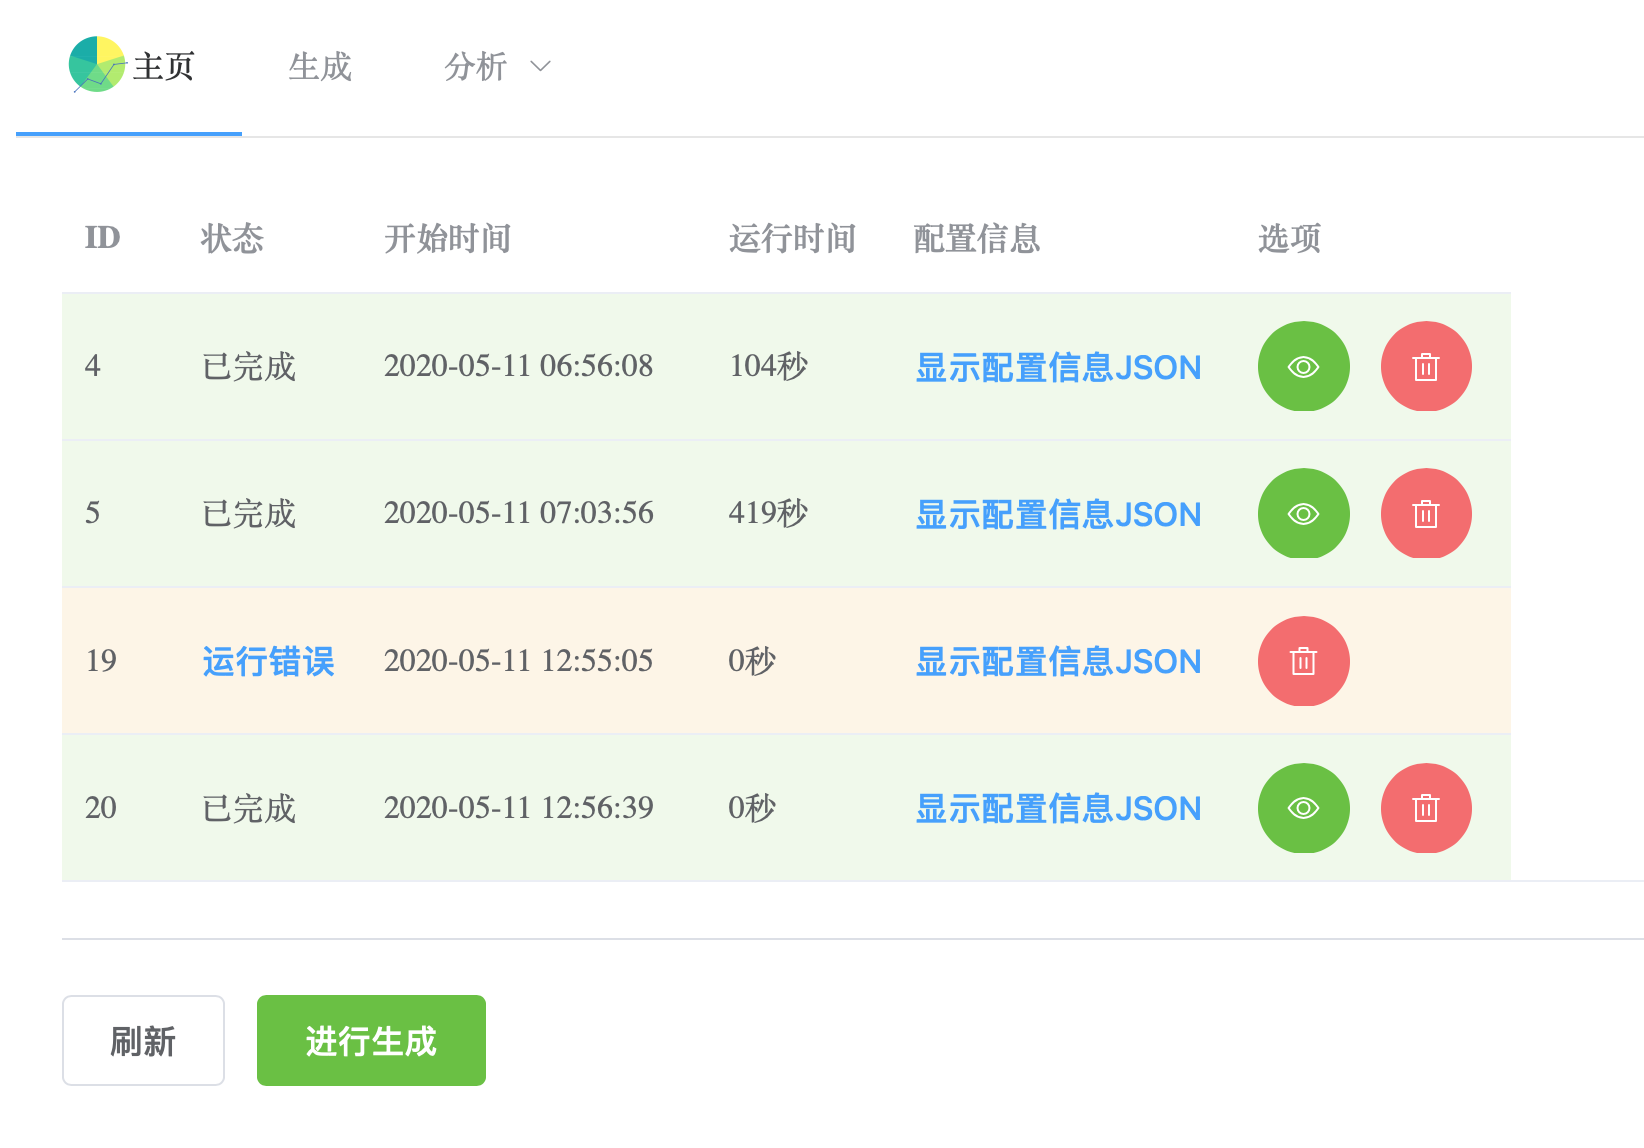
\includegraphics[scale=0.4]{frontend-home.png}
  \caption{管理系统-主页设计}
  \label{fig:frontend-home}
\end{figure}

在配置选择页面,用户可以用交互式操作进行每一个选项的详细配置。如图\ref{fig:iterations_node}、\ref{fig:edge_comm_event}所示。同时,也可以用JSON格式或者语句格式进行配置信息的导入。

\begin{figure}[H]
  \centering
  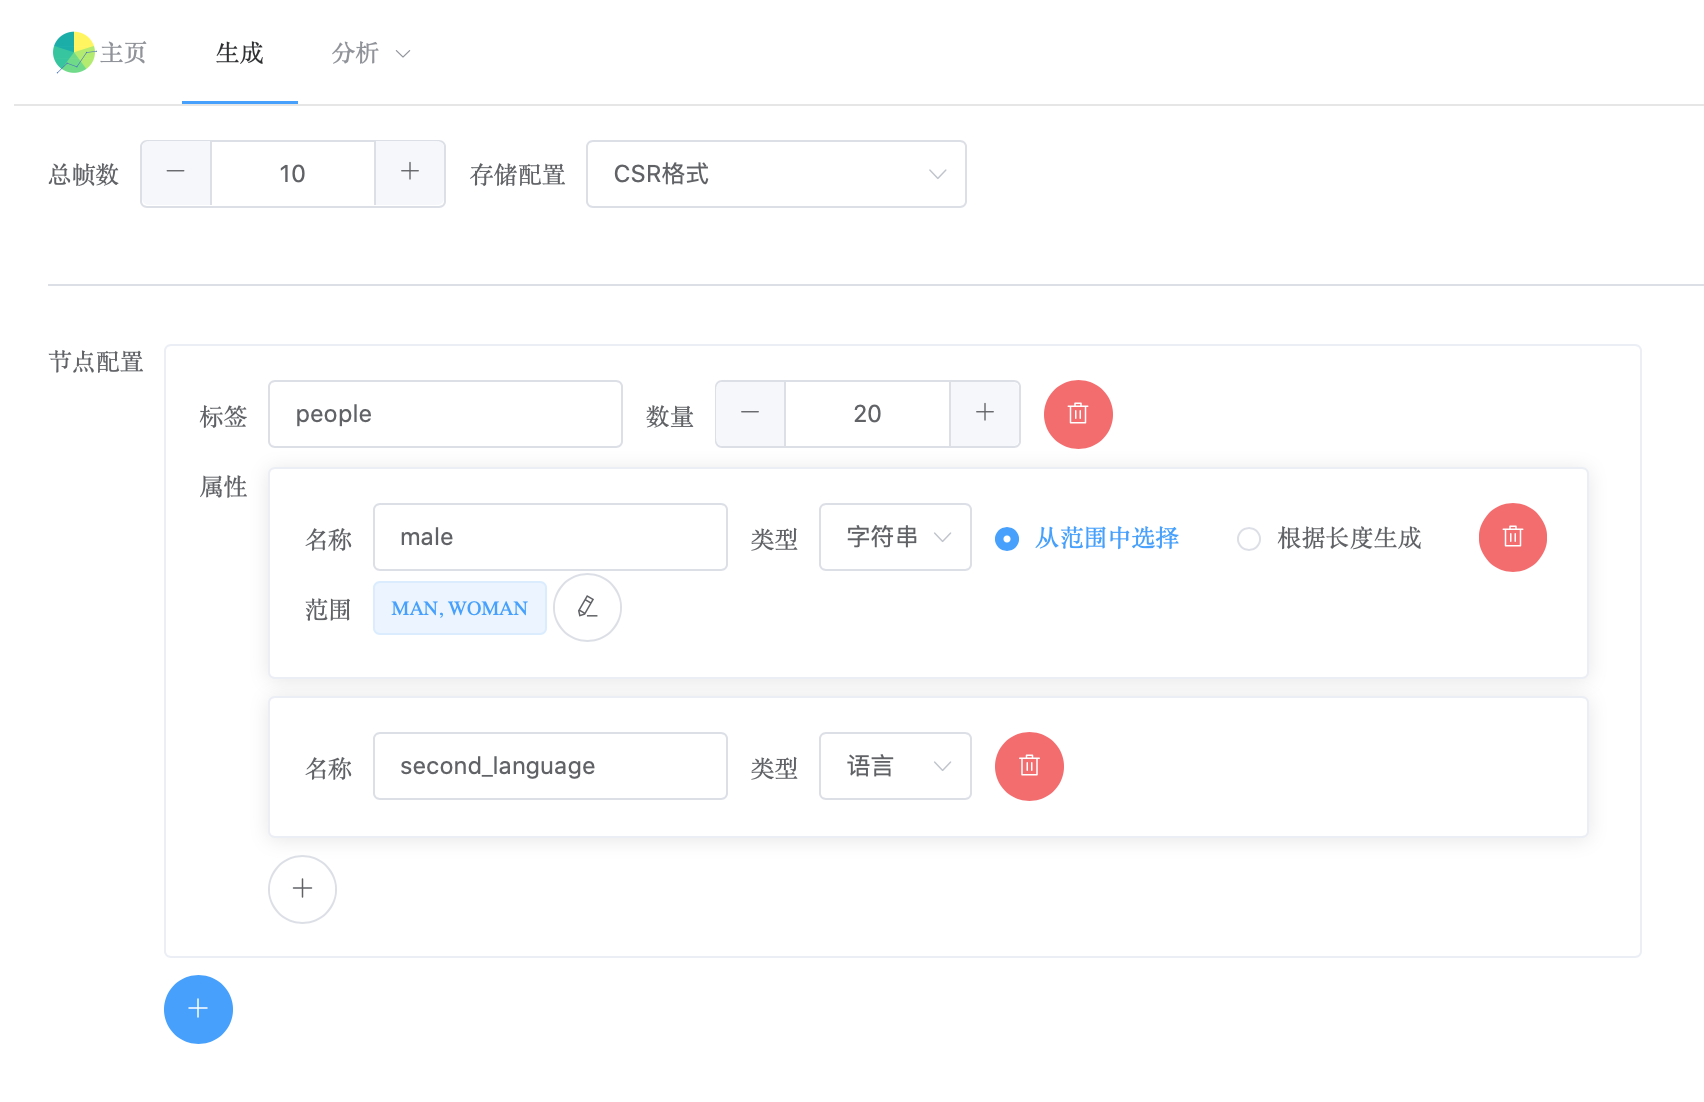
\includegraphics[scale=0.4]{iterations_node.png}
  \caption{管理系统-生成配置选项1}
  \label{fig:iterations_node}
\end{figure}

\begin{figure}[H]
  \centering
  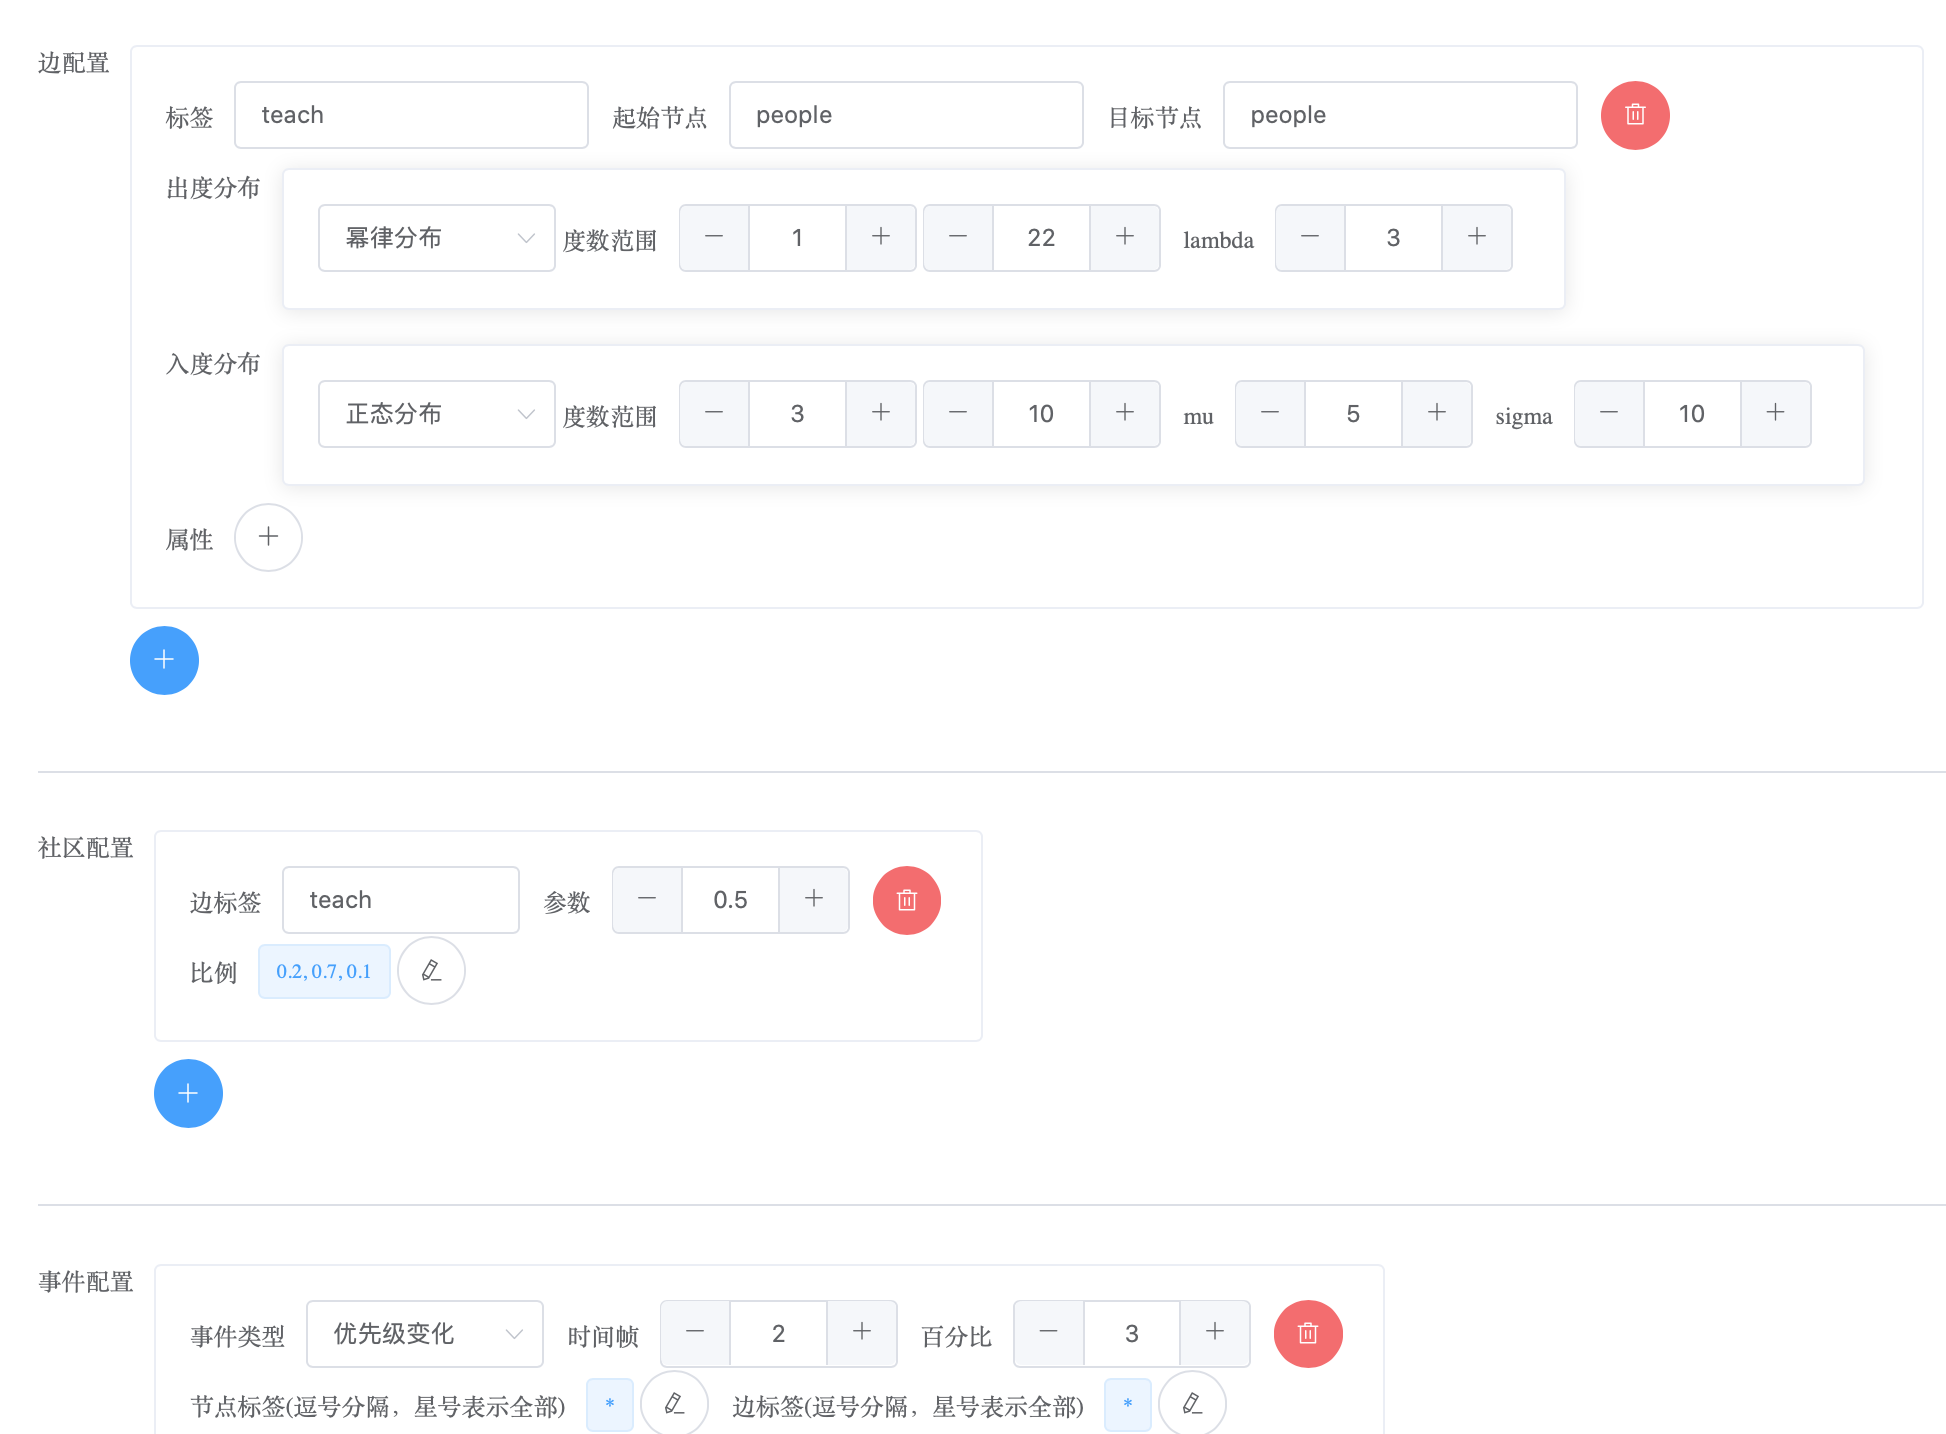
\includegraphics[scale=0.4]{edge_comm_event.png}
  \caption{管理系统-生成配置选项2}
  \label{fig:edge_comm_event}
\end{figure}

如图\ref{fig:analyzepage}所示,系统中实现了如下几种分析与可视化的显示:度数分布\footnote{度数分布部分展示每一个时刻对应的度数分布图}、度数变化\footnote{度数变化部分在选定一个节点,进行该节点度数变化分析}、节点变化\footnote{节点变化部分展示在各个事件中影响了哪些节点}、图可视化\footnote{图可视化部分会逐帧展示每一个时刻的图}。

\begin{figure}[H]
  \centering
  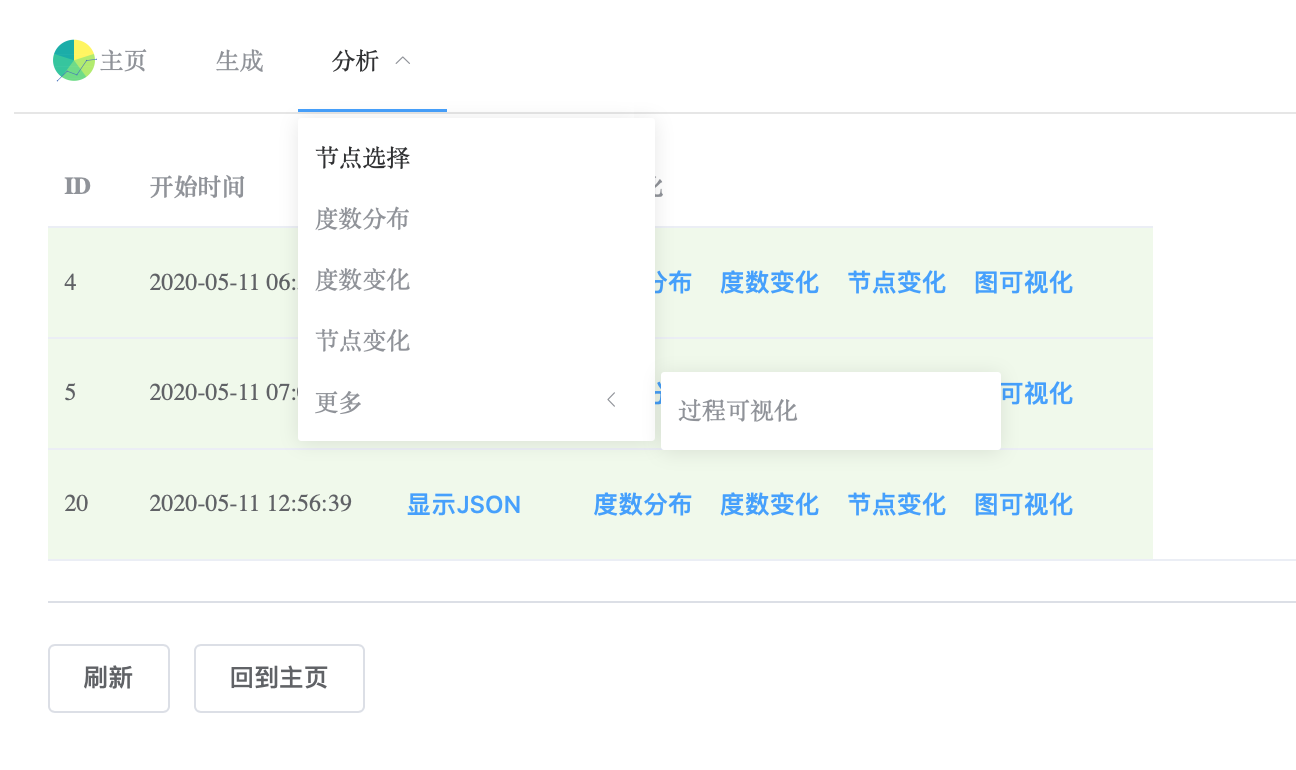
\includegraphics[scale=0.5]{analyzepage.png}
  \caption{管理系统-分析选项}
  \label{fig:analyzepage}
\end{figure}

以度数分布为例,其显示结果如图\ref{fig:degree_show}所示。选择边的标签、时刻信息、出度/入度分布之后,即可看到在这一个时刻的分布特征。

\begin{figure}[H]
  \centering
  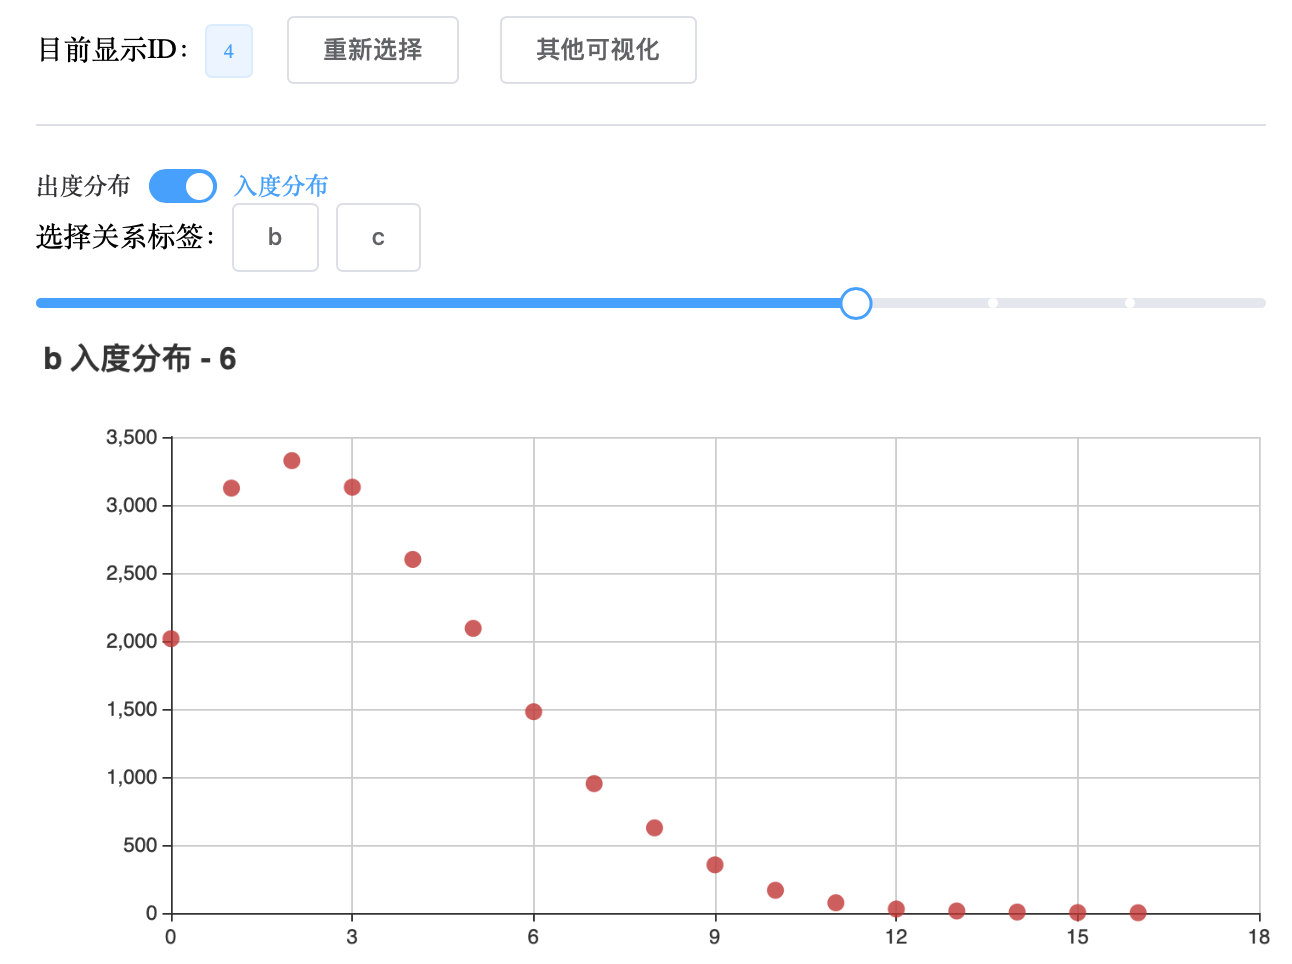
\includegraphics[scale=0.45]{degree_show.png}
  \caption{管理系统-度数分布分析}
  \label{fig:degree_show}
\end{figure}

\section{执行流程}

% 一个用户的典型操作过程与相应的前后端行为如下:

% \begin{enumerate}
%   \item 用户进入配置选择页面,进行所需动态图相关属性的配置(如图\ref{fig:iterations_node}、\ref{fig:edge_comm_event});
%   \item 前端将用户填写的配置信息转换为JSON格式,发送到后端;
%   \item 后端收到动态图生成请求与配置信息,分配一个新的线程进行生成操作,该线程会将生成任务相关信息存储到数据库中;
%   \item 用户获取生成结果,后端收到请求后在数据库中进行查询,若生成线程执行完成则将结果返回给前端进行结果的渲染与显示;
%   \item 用户选择进行可视化分析,后端收到请求后进行统计分析,将对应的结果返回前端进行渲染与展示。
% \end{enumerate}

% 具体执行流程如如图\ref{fig:stream}所示。

% \begin{figure}[H]
%   \centering
%   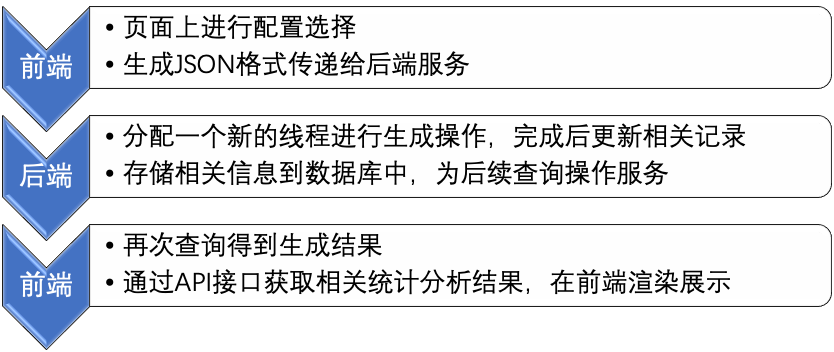
\includegraphics[scale=0.45]{stream.png}
%   \caption{管理系统-执行流程}
%   \label{fig:stream}
% \end{figure}

系统的具体执行流程如如图\ref{fig:uml_generate}与图\ref{fig:uml_analyze}所示。

\begin{figure}[H]
  \centering
  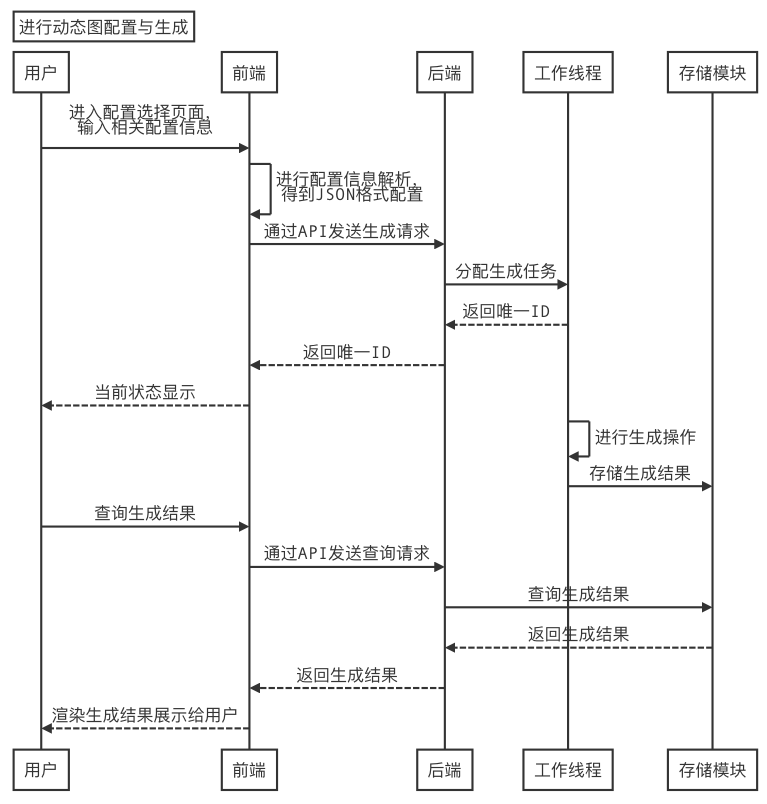
\includegraphics[scale=0.45]{uml_generate.png}
  \caption{动态图生成过程流程图}
  \label{fig:uml_generate}
\end{figure}

\begin{figure}[H]
  \centering
  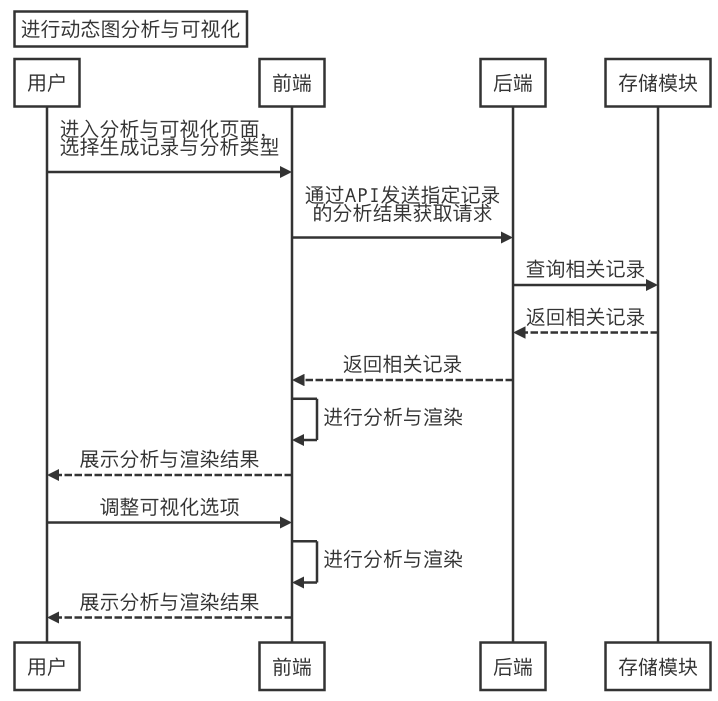
\includegraphics[scale=0.45]{uml_analyze.png}
  \caption{动态图分析与可视化流程图}
  \label{fig:uml_analyze}
\end{figure}

\section{本章小结}

本章对动态社交网络图生成管理系统的整体架构与执行流程进行了介绍。此系统中使用前后端分离的Restful架构设计,使用了第\ref{cha:chapter03}章中实现的动态社交网络图生成组件,用户可以方便地使用网页客户端进行配置选择、生成、历史记录查看与分析可视化等操作,极大地方便了用户的使用。